\documentclass{../industrial-development}
\graphicspath{{2-software-roles/}}

\title{Роли сотрудников в бизнес-процессах компании по разработке программного обеспечения.}
\author{Завойкин Алексей, ИТ-21 МО}
\date{}

\begin{document}

\begin{frame}
  \titlepage
\end{frame}

\begin{frame}{План лекции}
  \tableofcontents
\end{frame}

\section{Менеджер продукта }

\begin{frame} \frametitle{Менеджер продукта }
  
\end{frame}

\lecturenotes

Определение менеджера продукта часто напрямую зависит от определения менеджмента как такового. Менеджмент проекта – это совокупность знаний, навыков, инструментов и техник прилагаемых к проектным задачам с целью привести продукт к целям, поставленным заказчиком. Проектный менеджмент осуществляется через процессы инициирования, планирования, исполнения, наблюдения, контролирования и завершения. Проектный менеджер – человек, ответственный за выполнение всего вышеперечисленного. 
  ~\cite{Anatomy}
  
\begin{frame} \frametitle{Менеджер продукта: задачи}
  \begin{itemize}
  \item Установление критериев успеха
  \item Связь с клиентом
  \item Отслеживание статуса проекта
  \item Продвижение разработки вперед и преодоление проблем 
  \end{itemize}
\end{frame}

\lecturenotes

Менеджер продукта должен вовремя реагировать на потребности заказчика. Его главная задача — сформировать общее представление о поставленной задаче и о том, как ее решать. Он должен ответить на вопрос «Зачем мы делаем все это?» и убедиться, что все члены группы знают и понимают ответ на него.
Основная цель этой роли — удовлетворение требований заказчика. Для этого менеджер продукта выступает представителем заказчика в группе разработчиков и представителем группы у заказчика. (На этом этапе важно понимать разницу между заказчиком и пользователем: заказчик платит за создание продукта, а пользователи с ним работают.) Кроме того, менеджер продукта вместе с менеджером про­граммы должны прийти к компромиссному решению относительно функциональных возможностей продукта, сроков его разработки и финансирования проекта.
Как представитель заказчика, менеджер продукта отвечает за выполнение требований заказчика, создание бизнес-сценариев, формирование общего представления о проекте у группы и клиента, а также проверяет, удовлетворяют ли решения группы потребностям заказчика.
Как представитель группы, менеджер продукта отвечает за взаимодействие с заказчиком и управление его ожиданиями. При этом он проводит брифинги с клиентом и главными менеджерами, устраивает встречи с пользователями и демонстрации продукта.
Менеджер продукта сообщает группе предварительную дату выпуска продукта, устанавливаемую заказчиком. Однако в действительно успешных проектах графики составляются «снизу — вверх». При этом группа сама определяет возможную дату выхода приложения, которую менеджер продукта сообщает клиенту.
Группа менеджмента продукта представляет интересы заказчика и помогает ему определить необходимые функции приложения и их приоритеты. Отложить работу над какой-либо функцией вправе только заказчик, а переговоры по этим вопросам ведет менеджер продукта. За выполнение и составление графиков отвечает менеджер программы, поэтому в его власти изъять определенные функциональные возможности, чтобы текущая версия появилась в срок. Если менеджер программы решит сократить набор функциональных возможностей, чтобы не выбиться из графика,
он обязан сообщить об этом менеджеру продукта и заказчику, которые вправе согласиться или нет. В последнем случае заказчик и менеджер продукта должны согласовать изменение даты выпуска продукта. Кроме того, они могут увеличить финансирование с целью расширения состава группы. Затем менеджер программы определяет, как и на что потратить дополнительные деньги и поможет ли это выполнить план. Окончательное решение о финансировании принимают заказчик и менеджер продукта.
  ~\cite{Collective}

\begin{frame} \frametitle{Менеджер продукта: необходимая подготовка}
  \begin{itemize}
  \item Навыки функционального аналитика
  \item Навыки слушателя
  \end{itemize}
\end{frame}

\lecturenotes

Менеджеры продукта должны быть готовы выполнять определенную работу с постоянством. Должны быть готовы отступить от деталей и оценить проблемы целиком, готовы применить издержки личностного и командного характера. 
С целью сохранения рабочего процесса они также должны быть хорошими слушателями, чтобы убедиться, что проблема понята. 
Само заполучение роли зачастую спонтанно: архитектор решений или глава разработки выдвигает предложения по разработке и улучшению работы проекта, а также свою кандидатуру. Зачастую к роли приходят через роль функционального аналитика. 
  ~\cite{Anatomy}

\begin{frame} \frametitle{Менеджер продукта: инструментарий}
  \begin{itemize}
  \item Microsoft Project
  \item Шаблоны
  \end{itemize}
\end{frame}

\lecturenotes

ПО продукт-менеджера, такое как Microsoft Project или Microsoft Project Server, является важнейшим элементом инструментария. Оно помогает документировать зависимости, статус, что помогает отслеживать состояние проекта. 
Шаблоны – процесс менеджмента может стать крайне утомительным при переизбытки генерируемой документации. Инструменты, позволяющие убедиться в том, что процессы в разработке текут максимально эффективным способом, есть в инструментарии каждого менеджера. 
  ~\cite{Anatomy}

\begin{frame} \frametitle{Менеджер продукта: достоинства роли}
  \begin{itemize}
  \item Заметность работы
  \item Связь с начальством и другими проектными менеджерами
  \item Высокая степень влияния на продукт
  \item Подготовка к роли Senior lead
  \end{itemize}
\end{frame}

\begin{frame} \frametitle{Менеджер продукта: недостатки роли}
  \begin{itemize}
  \item Недостаток времени
  \item Переработка
  \item Не вовлечен непосредственно в разработку
  \item Работа сосредоточена на одном продукте в течение длительного времени
  \end{itemize}
\end{frame}

\lecturenotes

К позитивным элементам роли относят высокую заметность работника (связь с начальством и другими проектными менеджерами), степень влияния на продукт и удовлетворенность от вовлеченности в результаты работы. 
К негативным элементам – недостаток времени и переработку. 
  ~\cite{Anatomy}

\begin{frame} \frametitle{Менеджер продукта: связь с другими ролями}
  \begin{itemize}
  \item Функциональный аналитик
  \item Специалист по контролю качества
  \end{itemize}
\end{frame}
\lecturenotes
Карьерный рост продукт-менеджера возможен в двух направлениях:

Вертикальном стремлении к более высокой позиции — групп-продукт-менеджер, начальник отдела маркетинга, директор по маркетингу;
Горизонтальный переход к другой группе продуктов, который чаще практикуется в IT-сфере

\section{Специалист по контролю качества }

\lecturenotes

Специалист по контролю качества – роль работника, ответственного за обеспечение определенного уровня качества для финального клиента путём помощи команде разработки в определении проблем в процессе. Наиболее известным названием роли является понятие «тестировщик», но сама роль на тестировании не заканчивается  ~\cite{Anatomy}

\begin{frame} \frametitle{Специалист по контролю качества: задачи}
  \begin{itemize}
  \item Создание тестовых случаев и скриптов
  \item Отчетность о тестах
  \item Планирование тестов
  \item Случайное тестирование
  \item Выполнение скриптов и наблюдение за результатами 
  \end{itemize}
\end{frame}

\lecturenotes

Задачи специалиста сильно различаются в зависимости от проекта. Одни работники создают тестовые случаи и скрипты. Другие занимаются выполнением или наблюдением за этими случаями. Третьи специалисты занимаются «случайным» тестированием, чтобы убедиться, что в системе нет случайного «бага».   ~\cite{Anatomy}

Задача тестеров — испытание продукта в реальных условиях, дабы
определить, что в продукте работает и что не работает, и нарисовать таким образом точный «портрет» приложения. Естественно, для проведения тестов нужно отлично разбираться и в требованиях пользователей, и в том, как их удовлетворить.

Тестеры разрабатывают стратегию, планы, графики и сценарии
тестирования, которые позволяют убедиться, что все ошибки выявлены и исправлены до выпуска приложения. Ошибкой называют любую проблему, из-за которой продукт не выполняет свои функции. Ею может оказаться и ошибка в коде, называемая «жучком», и отклонение от спецификаций, заданных менеджером программы, и недоработки в документации, подготовленной группой обучения пользователей.

Важно различать тестирование и общую оценку качества, (Total Quality Assurance, TQA). Тестирование касается только проекта — точнее, его технической стороны. Проверку качества организует руководитель, ответственный за качество, — он выясняет соответствие продукта корпоративным, правительственным и другим стандартам.~\cite{Collective}

\begin{frame} \frametitle{Специалист по контролю качества: необходимая подготовка}
  \begin{itemize}
  \item Базовое понимание работы процесса
  \item Навыки в составлении документации
  \item Внимание к деталям
  \item Наблюдательность 
  \end{itemize}
\end{frame}

\lecturenotes

Роль специалиста – точка входа в сам процесс разработки. Необходимо лишь базовое понимание работы процесса, также приветствуется наличие опыта. 
Определенно, роль требует внимания к деталям, так что всё, что может продемонстрировать это внимание, необходимо специалистам по контролю за качеством. Так же высоко ценится наблюдательность и желание документировать результаты тестов. ~\cite{Anatomy}

\begin{frame} \frametitle{Специалист по контролю качества: инструментарий}
  \begin{itemize}
  \item Среда разработки
  \item Инструменты для автотестирования
  \item Инструменты для составления документации
  \end{itemize}
\end{frame}

\lecturenotes

Инструментарий специалистов заполнен инструментами, способными обеспечивать валидацию. Это включает в себя инструменты для автотестирования, и навыки, необходимые для проверки результатов работы, баз данных и даже рабочих потоков.  ~\cite{Anatomy}

\begin{frame} \frametitle{Специалист по контролю качества: достоинства роли}
  \begin{itemize}
  \item Вовлеченность в процесс
  \item Связь с проектом
  \item Имеет возможность импользовать автоматизацию тестирования
  \end{itemize}
\end{frame}

\begin{frame} \frametitle{Специалист по контролю качества: недостатки роли}
  \begin{itemize}
  \item Вопрос достаточности и избыточности
  \item Сообщение о плохих результатах работы непосредственно команде
  \item В обязанности входит больше, чем просто тестирование
  \end{itemize}
\end{frame}

\lecturenotes

К позитивным элементам относят вовлеченность в процесс: так как все элементы ПО должны быть протестированы, специалист оказывается вовлечен в процесс с ранних стадий. Кроме того, отмечается само качество работы: специалист способен максимально близко оценить продукт, над которым работает. 
К негативным элементам относят непростой вопрос достаточности и избыточности тестирования: вопрос того, насколько должен быть покрыт продукт тестами, возникает на каждом проекте и не имеет однозначного ответа. Кроме того, специалист сталкивается с необходимостью сообщать плохие новости команде.  ~\cite{Anatomy}

\begin{frame} \frametitle{Специалист по контролю качества: связь с другими ролями}
  \begin{itemize}
  \item Функциональный аналитик
  \item Архитектор решений
  \end{itemize}
\end{frame}
\lecturenotes
Специалист по контролю качества работает с функциональным аналитиком и архитектором решений чтобы превратить требования и документы в набор тестовых случаев и скриптов, которые будут использоваться для проверки. Набор этих документов называется тестовым планом.  ~\cite{Anatomy}

\section{Разработчик }

\lecturenotes

На самом базовом уровне разработчик – это работник, от которого ждут способности перевести алгоритмы и технические спецификации в код, который может быть исполнен на компьютере. Он должен знать синтаксис языка, однако на этом его знания ограничиваться не должны. Разработчик должен быть способен не только следовать указаниям при обучении новым технологиям и надстройкам, но и быть способен анализировать их, понимать, а также, при возможности, улучшать. Кроме того, так как в разработке ПО существует множество способов сделать одно и то же, разработчик должен обладать знаниями о структурах и алгоритмах, помогающих ему сделать это «правильнее».   ~\cite{Anatomy}

Разработчики знакомят остальных членов группы с применяемыми технологиями и собственно создают продукт. В качестве консультантов они предоставляют исходные данные для проектирования, проводят оценку технологий, а также разрабатывают прототипы и тестовые системы, необходимые для проверки решений и сокращения рисков на ранних стадиях процесса разработки. Чтобы создать продукт определенного качества, разработчикам не следует замыкаться на создании кода, они должны участвовать и в решении прикладной задачи. Они творят не ради творчества, а для реализации требований за­казчика. Часто, чтобы полностью разобраться в проекте, приходится создавать прототипы, а чтобы протестировать новую технологию, — испытательные системы, помогающие принять окончательное решение относительно архитектуры приложения. Этим также занимаются разработчики. ~\cite{Collective}
\begin{frame} \frametitle{Разработчик: задачи}
  \begin{itemize}
  \item Использование синтаксиса языка
  \item Анализ и понимание новых технологий
  \item Технологическое консультирование
\item Проектирование и осуществление реализации
\item Разработка приложений
\item Разработка инфраструктуры
  \end{itemize}
\end{frame}

\lecturenotes

Разработчик должен знать синтаксис языка, однако на этом его знания ограничиваться не должны. он должен быть способен не только следовать указаниям при обучении новым технологиям и надстройкам, но и быть способен анализировать их, понимать, а также, при возможности, улучшать. Кроме того, так как в разработке ПО существует множество способов сделать одно и то же, разработчик должен обладать знаниями о структурах и алгоритмах, помогающих ему сделать это «правильнее».   ~\cite{Anatomy}

Как программисты разработчики отвечают за низкоуровневое проектирование и оценку затрат на реализацию продукта. В большинстве организаций несколько основных разработчиков занимаются и архитектурой приложения. Как правило, это требуется на ранних ста­диях проекта, когда уточняются детали функциональных спецификаций и описывается взаимодействие продукта с внешними системами.

Разработчики сами оценивают сроки своей работы. Такая концепция MSF — создание графиков ответственными за выполнение конкретного участка членами группы — называется составлением расписания «снизу — вверх». Она позволяет выпустить нужный продукт в нужное время за счет уточнения графиков и повышения ответственности за выполнение работы в запланированные сроки.

Разработчики отвечают и за техническую реализацию проекта — в основном на фазах создания логической и физической модели. На этих стадиях их задача — определить методы реализации функциональных возможностей и заданной архитектуры, а также оценить сроки выполнения этой работы. Заметим, что разработчики не выбирают функции — они только решают, как их реализовать.

Кроме того, на стадии «Планирование» разработчики решают, какое влияние окажет на проект добавление или удаление некоторых функций. Разработчики не участвуют в заключительной стадии проекта — развертывании продукта, однако они должны тесно сотрудничать с логистиками на стадии установки приложения. ~\cite{Collective}
\begin{frame} \frametitle{Разработчик: необходимая подготовка}
  \begin{itemize}
  \item Навыки алгоритмиста 
  \item Знания о синтаксисе языка
  \end{itemize}
\end{frame}

\lecturenotes

Необходимая подготовка, в случае разработчика, является достаточно пугающим аспектом. Разработчик должен иметь навыки алгоритмиста и обладать знаниями синтаксиса языка. Самый популярный вопрос начинающих разработчиков – «какой язык я должен изучить?» Тот факт, что на этот вопрос не существует однозначного ответа, не делает языки равнозначными. Зачастую, язык зависит от области, в которой специалист хотел бы попробовать свои силы. 
Как и во многих отраслях, на собеседовании разработчик может столкнуться с работодателем, требующим наличие опыта. Однако это не должно остановить перспективного рекрута, ведь есть множество мест, где он мог бы набраться опыта, таких как некоммерческие организации или конкурсы по программированию. 
 ~\cite{Anatomy}

\begin{frame} \frametitle{Разработчик: инструментарий}
  \begin{itemize}
  \item Среда разработки
  \item Компилятор
  \item Отладчик
  \end{itemize}
\end{frame}

\lecturenotes

У разработчиков сравнительно небольшой инструментарий. От них ждут способности использовать различное окружение, включая компилятор и отладчик языка или языков, которые они выбрали. Кроме того, зачастую необходимо владеть полезными инструментами, популярными в команде разработчиков. 
В некоторых организациях от разработчика так же требуют быть знакомым с автоматизацией тестирования. Это включает в себя уровень unit-тестов, нацеленных на тестирование базовых вещей кода. 
  ~\cite{Anatomy}

\begin{frame} \frametitle{Разработчик: достоинства роли}
  \begin{itemize}
  \item Карьерный рост
  \item Стабильность
  \item Незаменимость
  \item Востребованность 
  \item Возможность выбора конкретной специализации
  \end{itemize}
\end{frame}

\begin{frame} \frametitle{Разработчик: недостатки роли}
  \begin{itemize}
  \item Вопрос личной замкнутости
  \item Зависимость от менеджмента
  \item Сравнительно высокие требования к образованию
  \item Большой объем работ
  \end{itemize}
\end{frame}

\lecturenotes

Карьерный рост отмечается как один из самых важных плюсов разработчиков. Так как область разработки – крупнейшая в сфере информационных технологий, существует множество специализаций и ролей, и практически всегда есть возможность продвинуться выше в иерархии. Роль разработчика является базовой ролью и может служить удачным трамплином к получению роли, скажем, ведущего разработчика или главы разработки.
Стабильность является также фактором, присущим разработчикам. Зачастую разработчики становятся незаменимы для работодателя, так как только они понимают, как устроена и работает программный продукт. Таким образом разработчики имеют надежное рабочее место даже во времена сокращений на проекте. 
Явными недостатками роли разработчика называют необходимость оставаться сосредоточенным на работе, приводящую к личностной замкнутости. Так же отмечается зависимость разработчиков от менеджмента проекта: неудачный решения могут привести к тому, что разработчик будет заниматься не свойственной ему работой, выполнять её некачественно и испытывать дискомфорт. 
  ~\cite{Anatomy}

\begin{frame} \frametitle{Разработчик: связь с другими ролями}
  \begin{itemize}
  \item Менеджер проекта
  \item Глава разработки
  \end{itemize}
\end{frame}
\lecturenotes
Как было сказано выше, менеджер проекта обладает значительными возможностями по установлению рабочего процесса разработчика. Сам же разработчик, при наличии необходимых знаний о проекте, личностных и профессиональных качеств, может получить роль главы разработки на проекте.  ~\cite{Anatomy}


\section{Архитектор решений }

\lecturenotes

Суть задач архитектора решений сводится к преобразованию требований к архитектуре и дизайну, который станет схемой создаваемого решения. Это преобразование основывается во многом на ранее уже созданные шаблоны, которые архитектор изучил ранее, или же с которыми столкнулся на практике, в реальных проектах. 
Сложность именно этих задач зачастую недооценивается. Всё это, в той или иной мере – форма искусства. Создание эффективных архитектур, позволяющих перейти непосредственно к реализации, должно выдерживать непростой баланс между концептами, варьирующимися от «Сохраняй простоту, глупый» (“Keep it simple, stupid”) до «Ошибка в сохранности» (“Fail to Save”).
   ~\cite{Anatomy}

\begin{frame} \frametitle{Архитектор решений: задачи}
  \begin{itemize}
  \item Преобразование требований к архитектуре
  \item стратегическое планирование технического развития системы
  \item Архитектурный надзор разработки
  \item Регламентация процедуры внесения изменений
  \item Разработка стандартов кодирования/проектирования
  \end{itemize}
\end{frame}

\lecturenotes

\begin{frame} \frametitle{Архитектор решений: необходимая подготовка}
  \begin{itemize}
  \item Знания о множестве технологий
  \item Богатый технический опыт
  \end{itemize}
\end{frame}

\lecturenotes
Другим переходом к роли архитектора может быть отход от роли главы разработки. Эти роли достаточно близки в навыках, которые требуются у работников. Архитектор выстраивает архитектуру для всего решения, в то время как глава разработки переводит это архитектуру в конкретный дизайн. 
Одним из путей, позволяющих продемонстрировать интерес к роли архитектора, является изучение паттернов. Так как именно их них строятся основные блоки в практически каждой архитектуре, их изучение может привести к тому, где именно они будут полезны. Также, необходимо расширение кругозора через чтение статей, ознакомление с новыми техниками, дабы увидеть возможности улучшения существующих архитектур. 
 ~\cite{Anatomy}

\begin{frame} \frametitle{Архитектор решений: инструментарий}
  \begin{itemize}
  \item Язык визуальной документации (UML)
  \item Средства для работы с БД
  \item Отладчик
  \end{itemize}
\end{frame}

\lecturenotes

Инструментарий архитектора больше чем у любого другого работника. Большинство архитекторов выросло в мире разработки ПО и обучилось работе с дюжиной инструментов, позволяющих повысить продуктивность. 
Возможно, самым важным инструментом в их наборе является язык визуальной документации, такой как UML. Структура UML, позволяющая описать множество различных видов разработки ПО наглядно, помогает оставаться этому языку оставаться самым известным языком визуальной документации. 
В дополнение к этому, архитектор должен быть сведущ в вопросах организации баз данных. В большинстве случаев ключ к успеху системы в целом зависит именно в успешной организации данных. 

  ~\cite{Anatomy}

\begin{frame} \frametitle{Архитектор решений: достоинства роли}
  \begin{itemize}
  \item Коммуникация с ключевыми работниками проекта
  \item Сравнительно невысокие требования к образованию 
  \item Высокая востребованность 
  \end{itemize}
\end{frame}

\begin{frame} \frametitle{Архитектор решений: недостатки роли}
  \begin{itemize}
  \item Тяжело уследить за новыми технологиями
  \item Сложный выбор между уже существующими технологиями
  \item Требуется дополнительная профессиональная подготовка
  \item Высокая степень ответственности 
  \end{itemize}
\end{frame}

\lecturenotes

Важными положительными чертами работы архитектора являются важность из позиции и возможность коммуникации с другими ключевыми работниками проекта, взаимный обмен опытом. В то же время, отмечается что архитектору тяжело уследить за всем: новые технологии появляются постоянно, как и инструменты. Так же, крайне тяжело выбрать правильный инструмент даже среди изученных и знакомых. 

  ~\cite{Anatomy}

\begin{frame} \frametitle{Архитектор решений: связь с другими ролями}
  \begin{itemize}
  \item Глава разработки
  \item Разработчик
  \end{itemize}
\end{frame}

\lecturenotes
Для большинства людей перехода к роли «Архитектора решений» просто-напросто не происходит. Это медленный, поступательный прогресс обучения и разработки. Человек может стать архитектором решений спустя несколько лет профессионального развития, но, как правило, этого не происходит в течение первого десятилетия. 
Отправной точкой является тот момент, когда разработчик остается единственным человеком на очень маленьком, зачастую совершенно не важном проекте. Возможно, достаточно маленьким, чтобы один человек выполнял все роли (в том числе, и роль архитектора). 
Другим переходом к роли архитектора может быть отход от роли главы разработки. Эти роли достаточно близки в навыках, которые требуются у работников. Архитектор выстраивает архитектуру для всего решения, в то время как глава разработки переводит это архитектуру в конкретный дизайн. 
Одним из путей, позволяющих продемонстрировать интерес к роли архитектора, является изучение паттернов. Так как именно их них строятся основные блоки в практически каждой архитектуре, их изучение может привести к тому, где именно они будут полезны. Также, необходимо расширение кругозора через чтение статей, ознакомление с новыми техниками, дабы увидеть возможности улучшения существующих архитектур. 

\section{Бизнес-аналитик }

\lecturenotes

В классическом понимании, бизнес-аналитик — это человек, который анализирует бизнес-потребности организации, а также формулирует пути и схемы усовершенствования бизнес-процессов, осуществляет стратегическое планирование. Бизнес-аналитики могут отвечать за одну конкретную сферу деятельности компании, либо за всю организацию в целом.   ~\cite{Business}

\begin{frame} \frametitle{Бизнес-аналитик: задачи}
  \begin{itemize}
  \item Усовершенствование продуктов компании
  \item Работа с клиентом
  \item Контроль над качеством продукта и соответствием требованиям клиента
  \item Формулирование высокоуровневых требований к программному продукту
  \item Составление его структуры и связей между элементами
\item Определение технологий и/или используемых программных решений
\item Проектирование юзер-интерфейса, формата и способа взаимодействия между пользователем и программой
  \end{itemize}
\end{frame}

\lecturenotes
Когда говорят о бизнес-аналитиках в IT, под их обязанностями, зачастую, подразумевают анализ и работу с требованиями к программным продуктам. В зависимости от рода деятельности компании, бизнес-аналитики могут выполнять одну из двух ролей:

Заниматься усовершенствованием продуктов компании — в случае, если она разрабатывает собственные решения. Чаще всего являются очень компетентными специалистами, но в наших краях (СНГ) встречаются намного реже, чем вторые.
Бизнес-аналитики в аутсорс и аутстаф компаниях — те люди, которых бросают на передовую работы с клиентами. Занимаются сбором требований, составлением ТЗ и многим другим. Далее речь пойдет именно о них.
Основной задачей бизнес-аналитиков в IT-аутсорс компаниях является работа с клиентом, а именно — контроль над тем, чтобы разрабатываемый продукт был качественным и полностью удовлетворял требованиям заказчика.
Являясь связующим звеном между заказчиком и командой разработки, бизнес-аналитик ведет клиента от начала и до конца работы над проектом. Он выясняет пожелания заказчика, его требования к продукту, консультирует его в спорных или технических вопросах, подсказывает пути решения поставленных задач.~\cite{Business}
 

\begin{frame} \frametitle{Бизнес-аналитик: необходимая подготовка}
  \begin{itemize}
  \item Новыки переговорищика
  \item Знания о технической стороне разработки ПО
  \item Эксперт в области проектирования интерфейсов 
  \item Знания о принципах движения денежного потока и работе с финансами 
  \item Навыки в области системного анализа
  \end{itemize}
\end{frame}

\lecturenotes
Таким образом, бизнес-аналитик должен быть компетентным в целом ряде не очень связанных между собой областей:

Быть хорошим переговорщиком (коммуникатором). Он должен уметь понять собеседника, объяснить ему сложные вещи из мира IT, убедить и переубедить клиента в эффективности разного рода решений, при необходимости — сгладить конфликтные ситуации;
Разбираться в технической стороне разработки ПО;
Обладать хотя бы базовой, но основательной экспертизой в юзабилити и проектировании интерфейсов;
Понимать принципы движения денежного потока и работы с финансами — чтобы иметь возможность до конца точно соблюсти интересы клиента относительно продукта, если разрабатывается коммерческое ПО;
Иметь прикладные навыки из области системного анализа: составление технической документации, специфических диаграмм и схем.

 ~\cite{Business}

\begin{frame} \frametitle{Бизнес-аналитик: инструментарий}
  \begin{itemize}
  \item Инструмент по агрегации всех рабочих задач
  \item Инструмент для поддержания ритма работы
  \item Инструмент коммуникации с проектной командой и заказчиком
  \end{itemize}
\end{frame}

  ~\cite{Business}

\begin{frame} \frametitle{Бизнес-аналитик: достоинства роли}
  \begin{itemize}
  \item Полное представление о проекте
  \item Определяющая развитие проекта деятельность
  \item Профессиональные качества можно перенести на другой род деятельности
  \end{itemize}
\end{frame}

\begin{frame} \frametitle{Бизнес-аналитик: недостатки роли}
  \begin{itemize}
  \item Сложности в общении с заказчиком
  \item Изучение больших объемов информации в сжатые сроки
  \item Необходимость постоянного обучения новым подходам и методологиям
  \item Дедлайны могут привести к увеличению рабочего времени 
  \end{itemize}
\end{frame}

\lecturenotes

Главное преимущество профессии бизнес-аналитика — возможность проникать в суть: разбираться, что как устроено, из каких частей состоит, как они между собой связаны и взаимодействуют, и затем описывать сложные вещи с помощью простых, но полезных моделей. Бизнес-аналитики помогают разным сторонам понимать друг друга, и в результате получают реализацию, которая удовлетворит всех. Еще один плюс — важность и значимость деятельности, так как именно результаты работы бизнес-аналитика определяет ход проекта. Среди недостатков выделяют сложности в общении с заказчиком, когда не удается донести хорошие идеи или же мешают ограничения в сроках и бюджете. Другая жалоба — необходимость изучать большие объемы информации в краткие сроки. Кроме изучения непосредственно своего проекта, бизнес-аналитик обязан постоянно держать руку на пульсе новых методологий, подходов, изучать базовые принципы новых платформ.

  ~\cite{Business}

\begin{frame} \frametitle{Бизнес-аналитик: связь с другими ролями}
  \begin{itemize}
  \item Проектный менеджер
  \item Продукт-менеджер
  \item Архитектор решений
  \end{itemize}
\end{frame}

\lecturenotes 
Можно выделить 2 пути становления: 
IT-специалист, которому ближе общение, чем написание кода. Такой аналитик будет понимать процесс разработки, знает возможности ПО и понимает, что нужно знать разработчику для качественной работы. Однако ему необходимо отдельно приобретать бизнес-знания в области, которая автоматизируется;
Специалист без IT-образования, который является профессионалом в определенной предметной области. Такой аналитик понимает все нюансы бизнеса и разговаривает с заказчиком на одном языке. Но ему придется разбираться, что именно подлежит автоматизации и какие данные нужны разработчикам для работы;
Перспективы карьерного развития бизнес-аналитика: 
Совершенствоваться как аналитик, осваивать все больший круг аналитических задач;
Углубиться в системную составляющую и стать Business или Enterprise Architect; 
Развиваться по управленческой лестнице, проектной (Project manager -> Program Manager -> CTO) или бизнес (Product manager); 
Перспективы разные. Стать руководителем подразделения аналитики, стать квалифицированным специалистом, предоставлять консалтинговые услуги. Даже открывая свое дело, необходимо анализировать рентабельность бизнеса. И в уже созданном бизнесе необходимо анализировать и прогнозировать результаты работы.~\cite{Business}

\begin{frame} \frametitle{Общая схема связи ролей в разработке ПО}
 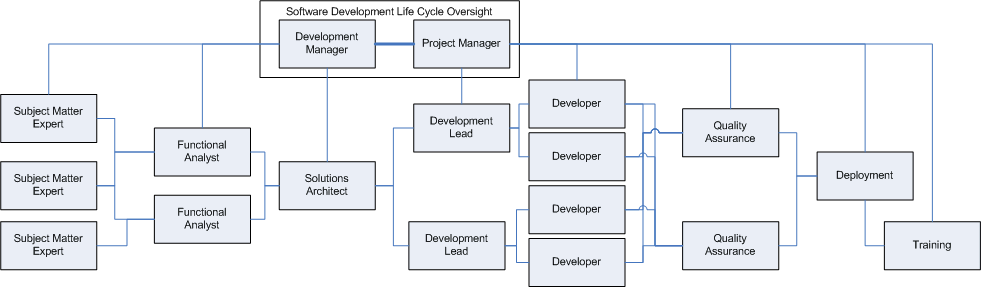
\includegraphics[width=\textwidth]{Fullorgchart1}

\end{frame}


\section{Группы ролей}

\begin{frame} \frametitle{Группы ролей}
  \begin{itemize}
    \item Анализ. 
    \item Извлечение, документирование и сопровождение требований к продукту.
    \item Управление. 
    \item Определение и управление производственными процессами.
    \item Производство.
  \end{itemize}
\end{frame}

\begin{frame} \frametitle{Группы ролей}
  \begin{itemize}
    \item Проектирование и разработка ПО.
    \item Тестирование. 
    \item Тестирование ПО.
    \item Обеспечение. 
    \item Производство дополнительных продуктов и услуг.
\end{frame}

\begin{frame} \frametitle{Общая схема связи ролей в разработке ПО}
 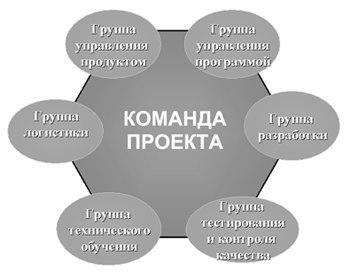
\includegraphics[width=\textwidth]{projectteam}

\end{frame}

\subsection{Группа анализа}

\begin{frame} \frametitle{Бизнес-аналитик}
Построение модели предметной области (онтологии).
\end{frame}

\begin{frame} \frametitle{Бизнес-архитектор}
Разрабатывает бизнес-концепцию системы. Определяет общее видение продукта, его интерфейсы, поведение и ограничения.
\end{frame}

\begin{frame} \frametitle{Системный аналитик}
Отвечает за перевод требований к продукту в функциональные требования к ПО.
\end{frame}

\begin{frame} \frametitle{Специалист по требованиям}
Документирование и сопровождение требований к продукту.
\end{frame}
 
\begin{frame} \frametitle{Функциональный заказчик}
Представляет в проекте интересы пользователей продукта.
\end{frame}
 
\subsection{Группа управления}
\begin{frame} \frametitle{Руководитель проекта}
Отвечает за достижение целей проекта при заданных ограничениях (по срокам, бюджету и содержанию), осуществляет операционное управление проектом и выделенными ресурсами.
\end{frame}

\begin{frame} \frametitle{Куратор проекта}
Оценка планов и исполнения проекта. Выделение ресурсов.
\end{frame}

\begin{frame} \frametitle{Системный архитектор}
Разработка технической концепции системы. Принятие ключевых проектных решений относительно внутреннего устройства программной системы и её технических интерфейсов.
\end{frame}

\begin{frame} \frametitle{Руководитель группы тестирования}
Определение целей и стратегии тестирования, управление тестированием.
\end{frame}

\subsection{Другие группы}

\begin{frame} \frametitle{Производственная группа}
  \begin{itemize}
    \item Проектировщик. 
    \item Проектировщик базы данных.
    \item Проектировщик интерфейса пользователя.
    \item Разработчик.
  \end{itemize}
\end{frame}

\begin{frame} \frametitle{Группа тестирования}
  \begin{itemize}
    \item Проектировщик тестов.
    \item Тестировщик.
  \end{itemize}  
\end{frame}

\begin{frame} \frametitle{Группа обеспечения}
  \begin{itemize}
  \item Технический писатель.
  \item Переводчик.
  \item Дизайнер графического интерфейса.
  \item Разработчик учебных курсов, тренер.
  \item Участник рецензирования.
  \end{itemize}  
\end{frame}

\begin{frame} \frametitle{Группа обеспечения}
\begin{itemize}
  \item Продажи и маркетинг.
  \item Системный администратор.
  \item Технолог.
  \item Специалист по инструментальным средствам.
  \end{itemize}  
\end{frame}


\begin{frame} \frametitle{Совмещение и разделение ролей}
Зависит от масштаба проекта. Одну роль могут исполнять несколько человек.
\end{frame}


Зависит от масштаба проекта. Одну роль могут исполнять несколько человек. Например: разработчики, тестировщики, технические писатели.
Один человек может исполнять несколько ролей. Некоторые роли может исполнять только один человек. Например, Руководитель проекта, Системный архитектор.

\begin{frame} \frametitle{Возможно совмещение ролей:}
\begin{itemize}
\item Руководитель проекта + Системный аналитик (+ Системный архитектор)
\item Системный аналитик + Проектировщик тестов (+ Технический писатель)
\item Системный аналитик + Проектировщик интерфейса пользователя
\item Ответственный за управление конфигурациями + Ответственный за сборку и поставку (+ разработчик)
\end{itemize}  
\end{frame}

\begin{frame} \frametitle{Не рекомендуется совмещение ролей:}
\begin{itemize}
\item Руководитель проекта + Разработчик)
\item Разработчик + Системный аналитик.
\item Разработчик + Проектировщик интерфейсов пользователя.
\item Разработчик + Тестировщик
\end{itemize}  
\end{frame}

\begin{thebibliography}{99}

\bibitem{Anatomy} \href{https://www.developer.com/tools/article.php/3526491/}{Anatomy of a Software Development Role}
\bibitem{Business} \href{https://itkeys.org/business-analysts/}{Бизнес-аналитики в IT}
\bibitem{Collective} \href{http://vit-prog.narod.ru/page/TRPP/section_3/subjec_3.2.htm}{Коллективная разработка ПО}
\end{thebibliography}

\end{document}
%%% Local Variables: 
%%% mode: TeX-pdf
%%% TeX-master: t
%%% End: